\documentclass[a4paper,UKenglish,cleveref, autoref]{lipics-v2019}
% \documentclass[preprint, 10pt, numbers]{sigplanconf}
% \documentclass[9pt,preprint]{sigplanconf}
% \documentclass[pldi,10pt,preprint]{sigplanconf-pldi16}

% The following \documentclass options may be useful:

% preprint      Remove this option only once the paper is in final form.
% 10pt          To set in 10-point type instead of 9-point.
% 11pt          To set in 11-point type instead of 9-point.
% authoryear    To obtain author/year citation style instead of numeric.

\usepackage{graphicx}
\usepackage{caption}
\usepackage{subcaption}

\begin{document}

% \newcommand{\charcoal}{Charcoal}
\newcommand{\charcoal}{DblBlind}
\newcommand{\atomic}{\texttt{atomic}}

\special{papersize=8.5in,11in}
\setlength{\pdfpageheight}{\paperheight}
\setlength{\pdfpagewidth}{\paperwidth}

% \doi{nnnnnnn.nnnnnnn}

\title{To Async or Not to Async? Better Cooperative Multithreading is the Answer}
\titlerunning{To Async or Not to Async?}

\author{Double Blind} {Double Blind, [optional: Address], Country \and \url{http://double.blind} } {double@blind} {https://orcid.org/double-blind} {(Optional) author-specific funding acknowledgments}
% \author{Benjamin Ylvisaker} {Colorado College, [optional: Address], Country \and \url{http://www.myhomepage.edu} } {bylvisaker@coloradocollege.edu} {https://orcid.org/0000-0002-1825-0097} {(Optional) author-specific funding acknowledgments}

%% \authorinfo{Blind Review}
%%            {Blind Review University}
%%            {BlindReview@BlindReview.edu}

\authorrunning{D. Blind}

\maketitle

\begin{abstract}

For many years events and their close cousins were the most widely used intra-process multitasking abstraction.
In the last decade (or so), many mainstream languages have implemented some flavor of coroutine, and their use has risen dramatically.

Coroutines are superior to events in some important ways, but they still have their weaknesses.
In this paper we analyze some of the software engineering problems related to coroutines and advocate for cooperative multithreading as a better alternative.

Our primary problem with coroutines is that the important choice between atomic and interruptible for procedure-like abstractions is made by the author, not the caller.
We present evidence that, though not a crisis, this issue does cause problems in practice.

Existing implementations of cooperative multithreading have weaknesses relative to coroutines.
Two important ones are not knowing or being able to control the atomicity of procedures at call sites, and the efficiency of call frame allocation.
We propose a new flavor of atomic block and a new call frame allocation strategy to address these issues.
With these improvements, we believe that cooperative threads represent a better alternative to coroutines.

\end{abstract}

% \category{CR-number}{subcategory}{third-level}

% general terms are not compulsory anymore,
% you may leave them out
% \terms
% term1, term2

% \keywords
% keyword1, keyword2

%% Why Events, Preemptive Threads and Coroutines are All Bad Ideas\footnotemark
%% \footnotetext{This tongue-in-cheek subtitle is a reference to Ousterhout \cite{Ousterhout1996} and von Behren, et al. \cite{Behren2003a}}






problems with coroutines:









\section{Introduction}

A generation ago (give or take) there was a wide-ranging debate about the relative merits of multithreading and event loops for intra-process multitasking (a.k.a. asynchronous programming).
It is interesting to note that a couple of the best-known contributions to the discussion (\cite{Ousterhout1996} and \cite{Behren2003a}) are both framed negatively.
That is, they both focus on what is wrong with the \emph{other} solution.

And there is plenty to criticize about both multithreading and event loops.
To mention just a couple of the most important software engineering problems, multithreading makes avoiding concurrency bugs far too hard \cite{Lu2008} and event loops force programmers to write far too much boilerplate code for non-trivial multitasking patterns \cite{Adya2002} (colloquially called \emph{callback hell}).

Nevertheless, multitasking is an unavoidable facet of most applications.
In many mainstream application domains, where the parallelism offered by multithreading was not important, event loops became the most common solution.
In recent years the richness of multitasking in many application domains has increased along with a few trends: increasing use of network services (e.g. Web APIs), increasingly rich physical world interaction (especially on mobile devices), and the increasing use of multi-process software architectures (e.g. microservices).
This has put renewed pressure on programming languages to provide good ways to write robust, maintainable and efficient multitasking code.

Many popular languages have recently introduced or expanded support for coroutines, as an alternative to event loops.
Coroutines are certainly an improvement in important ways.
However, coroutines still have problems.
In particular, in this paper we focus on the fact that there are many common library procedures that should be atomic in some calling contexts and interruptible (i.e. asynchronous) in others.
Coroutines force library authors to make the choice between atomic and interruptible and do not provide an easy way to override the choice in either direction.

We believe that cooperative multithreading is a better option for many applications.
Of course, cooperative multithreading has been widely understood for decades, and was surely an alternative that language designers considered when they chose coroutines.
Traditional implementations of cooperative multithreading have had some important disadvantages relative to coroutines.
Two that we aim to mitigate in this paper are:
\begin{itemize}
\item Call frame allocation efficiency
\item Visibility and control of atomicity
\end{itemize}

We introduce a new call frame allocation strategy called \emph{hot stacking} that is both space and time efficient, at the expense of some code management complexity.
We adapt work on atomic blocks from the parallel{\slash}preemptive multithreading domain to give programmers control over atomicity.
With these improvements, we believe that cooperative multithreading is a strict improvement over coroutines in many contexts.

\subsection{Multitasking, Not Parallelism}

Multitasking is, of course, a cousin of parallelism.
In this paper we focus entirely on the former.
Our work on call frame allocation shares at least some similarities with efforts to make parallel{\slash}preemptive multithreading more lightweight (e.g. the Java Loom project \cite{Pressler2017}).
We believe that it is better to design different language features for multitasking and parallelism; C\# is a good example of this philosophy, with async{\slash}await for multitasking and easy integration with worker thread pools for parallelism.

\section{Background: Coroutines and Cooperative Multithreading}

Coroutines have been used in various forms for a long time.
Perhaps the earliest published reference is from a 1963 compiler paper \cite{Conway1963}.
Modula-2 had coroutines as a standard language feature in the 1980s.
Felleisen and Hieb \cite{Felleisen1992} gave a good theoretical treatment of continuations, which have been used widely as a formal foundation for coroutines.

Coroutines played a relatively small role in mainstream programming practice until the last ten years or so.
Popular ``scripting'' languages introduced coroutines to a much wider audience.
For example, some flavor of coroutines were added to Lua in version 5.0, Python in version 2.5 and Ruby in version 1.9.
de Moura and Ierusalimschy \cite{Moura2009} gave a nice account of the many subtle variations on coroutines and advocated for their more general use.
C\#{\slash}.Net got on the bandwagon in 2012 with async{\slash}await.
JavaScript now has native syntax for both major flavors of coroutines (generator and async function).
Even the staid C++ community is considering standardizing support for coroutines (though the relevant proposals have been making their way through the committee process relatively slowly).

\subsection{The Coroutine Menagerie}

Coroutine-like abstractions come in a number of different flavors, which makes them easy to miscommunicate about.
The essential feature of coroutines is that they can invoke a \emph{yield{\slash}await} primitive to suspend their own execution and resume the execution of some other suspended coroutine.
In language designs with coroutines, typically routines{\slash}procedures{\slash}functions{\slash}methods are defined to be either regular routines or coroutines.
An extremely important distinction between flavors of coroutines is whether it is legal to invoke yield from a regular subroutine called by a coroutine.
This distinction is sometimes referred to as ``stackful'' versus ``stackless'' coroutines.
Some sources use ``coroutine'' to refer to the stackful variant and ``semi-coroutine'' for the stackless one.
Most modern implementations are stackless, so we will use ``coroutine'' to refer to this variant.
Stackful coroutines are essentially equivalent to cooperative multithreading, which is discussed below.

``Calling'' a coroutine is quite different from a regular routine call.
Calling a coroutine spawns a new dynamic instance of that coroutine and returns a handle{\slash}reference to that instance\footnotemark{}.
The two major patterns for coroutine use are defined by what can be done with this handle.
Generator-style coroutines allow sequences of values to be passed in to and back out of the coroutine.
These sequences of values manifest as inputs to and outputs from yield.
Async-style coroutines only allow the caller to wait for the final return value from the coroutine instance.
Unlike a regular subroutine call, during the execution of the coroutine, control may transfer to some other concurrent coroutine.

\footnotetext{In some older designs, there could only be one dynamic instance of a particular coroutine, and subsequent calls would advance the state to the next yield.
This inflexible design is not used by any modern implementations we are aware of.}

Some languages have distinct primitives for these two styles.
For example, JavaScript has both \texttt{function*} (generator) and \texttt{async function}.
The difference between the two is superficial.
A language with generator-style coroutines can support async-style with a simple adapter function that loops internally until the generator is finished.
A language with async-style coroutines can support generator-style with a simple adapter function that creates a one-deep bidirectional queue that can be used to pass sequences of values in and out.

In practice async-style is the more commonly used pattern, so it is what we focus on in this paper.
Other patterns certainly have their place, and they are not incompatible with anything we propose.

\subsection{Immediate Waiting is More Common}

When a coroutine is called, the caller can either immediately wait for the result, or it can store the handle and do some other work before waiting on the handle.
The latter case creates concurrency between the callee and the caller, and possibly other coroutines that either goes on to call.
In practice it is more common for the caller to immediately wait for the result of the callee.
This means that basic interface going on is that of a regular subroutine call, with the essential difference that the call might be interrupted before returning.
We refer to this pattern as calling an interruptible subroutine, in contrast to calling a regular atomic subroutine.

This conclusion is based on examining 60 of the most popular public projects written in JavaScript, based on NPM most-depended-upon and Github most-starred lists.
Many of these projects do not use async{\slash}await at all, in some cases surely because the project predates the language feature.
In these projects, of the 1615 lines that use await, approximately 84\% appear to be awaiting directly on a call to some application function.
Approximately 3\% involve the Promise library (for example \texttt{Promise.all}).
Approximately 13\% are something else, like awaiting on a variable.
For this analysis we filtered out files that appeared to be for internal testing purposes; some of these files included trivial expressions like \texttt{await 1} that we do not consider to be representative of regular application code.

%    1357 calls 84
%      50 promise 3
%     208 other 13
%    1615

\subsection{Cooperative Multithreading}

Like coroutines, cooperative multithreading is an old idea that has been interpreted in a variety of subtly different ways.
Because we are interested in the differences between coroutines and cooperative multithreading, we provide an informal sketch of a definition of the latter by translation to the former.
Given a target language with async-style coroutines, cooperative multithreading can be defined in a source language by translating \emph{all} routines to coroutines in the target.
All normal routine calls in the source language have an implicit await inserted in the translation.
Spawning new cooperative threads is translated to a regular call without an inserted await.
Yield{\slash}await can be invoked anywhere, as is usual in cooperative multithreading, because all code is effectively in an async routine.

This translation sketch highlights the two problems with cooperative multithreading that we aim to mitigate in this paper.
First, all calls, even to very short-lived routines, are ``async calls''.
This has important efficiency implications that we discuss in more detail later.
Second, there is no indication at call sites whether the called routine will yield or not.
This is in contrast to coroutines, where calls to potentially interruptible routines are clearly marked with await or yield.
This has an impact on programmer reasoning about atomicity properties and related potential concurrency bugs.

\section{Problems with Coroutines}

As mentioned previously, we believe coroutines are a reasonably good multitasking primitive.
But there is room for improvement.

\subsection{Atomic vs Interruptible Library Duplication}

When a library author wants to make a procedure-like abstraction, they have to choose between making it an atomic routine or an interruptible coroutine.
(Of course it is possible to provide both, a topic we will return to shortly.)
For many routines the choice between atomic and interruptible seems obvious.
If a routine does a fixed amount of computational work and does not interact with the outside system, it should almost certainly be atomic.
If a routine might take a lot of time, or interacts with the outside system in a nontrivial way, it should be an interruptible coroutine.

Unfortunately, many routines fall in the awkward middle ground where in some calling contexts they should be atomic and in others they should be interruptible.
One case that is easy to see in this middle ground is any routine that takes an arbitrary amount of data as a parameter and does work proportional to the size of the data.
When the amount of data is small, the routine completes quickly and it is best for the whole call to be atomic.
When the amount of data is large, the routine might take a long time and should be interruptible to avoid unresponsiveness.

Providing essentially duplicates of the same routine to give the caller the choice between atomic and interruptible violates the Don't Repeat Yourself software engineering rule of thumb.
Nevertheless, this pattern can be seen even in widely used standard libraries.
In the node.js standard library there are 50 function names that have a \texttt{[name]Sync} copy; in the C\#{\slash}.Net standard library there are 208 method names that have a \texttt{[name]Async} copy.
The majority of these duplicate functions have names that suggest they are related to filesystem, network or process control operations.
The next most common subset of these duplicates have names that suggest data processing like compression and encryption.
This duplication exists in spite of specific recommendations to avoid it (for example, from the Microsoft developer blog: \cite{Toub2012, Toub2012a}).

We do not want to overstate the problem.
These standard libraries have thousands of functions; the duplicates represent a small fraction.
Nevertheless, their existance in some of the most widely used and actively maintained libraries in the world indicates a problem.

% 35 FS  chownSync utimesSync rmdirSync truncateSync lchmodSync fdatasyncSync lchownSync fchmodSync renameSync appendFileSync closeSync futimesSync readdirSync readFileSync mkdirSync symlinkSync fstatSync statSync mkdtempSync readSync accessSync fchownSync readlinkSync chmodSync copyFileSync writeFileSync ftruncateSync linkSync fsyncSync unlinkSync lstatSync realpathSync openSync writeSync existsSync
%  3 Proc  execSync spawnSync execFileSync
% 10 Data  deflateRawSync generateKeyPairSync unzipSync pbkdf2Sync inflateSync deflateSync inflateRawSync gunzipSync gzipSync randomFillSync
%  2 ?  maybeSync scryptSync

% 21 Net ConnectAsync GetHostAddressesAsync SpeakAsync GetPageAsync AddOnMapRequestHandlerAsync AddOnLogRequestAsync ReceiveFromAsync PutAsync DownloadFileAsync GetPageRootAsync DownloadDataTaskAsync AcceptAsync AnnounceOfflineTaskAsync PatchAsync WriteToServerAsync GetResponseAsync CancelConnectAsync AuthenticateAsClientAsync AcceptTcpClientAsync GetClientCertificateAsync DisconnectAsync
% 72 FS ReadElementContentAsBase64Async ReadAsByteArrayAsync ReadContentAsObjectAsync ReadElementContentAsStringAsync CreateContactAsync WriteEndDocumentAsync LoadGrammarAsync GetMetadataAsync WriteBinHexAsync AppendAllTextAsync GetHostEntryAsync ReadLineAsync ReadElementContentAsAsync ReadAsync AppendAllLinesAsync WriteAllLinesAsync ReadAllLinesAsync ReadElementContentAsObjectAsync ReadAsStreamAsync ReadOuterXmlAsync ReadBlockAsync ReadContentAsAsync ReadElementContentAsBinHexAsync CreateContentReadStreamAsync ReadToEndAsync ReadAllBytesAsync ReadValueChunkAsync ReadContentAsStringAsync ReadContentAsBinHexAsync WaitToReadAsync ExecuteXmlReaderAsync ReadContentAsBase64Async ReadAllTextAsync ReadInnerXmlAsync OpenReadAsync ExecuteDbDataReaderAsync ExecuteReaderAsync ReadAsStringAsync ReadFromAsync WaitForConnectionAsync WriteNameAsync WriteToAsync WaitToWriteAsync WriteCDataAsync WriteNmTokenAsync WriteElementStringAsync WriteStartElementAsync WriteLineAsync WriteSurrogateCharEntityAsync WriteEndElementAsync OpenWriteAsync WriteRawAsync WriteStringAsync WriteWhitespaceAsync WriteAllBytesAsync WriteEndAttributeAsync WriteCommentAsync WriteBase64Async WriteAsync WriteProcessingInstructionAsync WriteAllTextAsync WriteAttributeStringAsync WriteEntityRefAsync WriteCharsAsync WriteFullEndElementAsync WriteStartDocumentAsync WriteNodeAsync WriteDocTypeAsync WriteStartAttributeAsync WriteQualifiedNameAsync WriteAttributesAsync WriteCharEntityAsync
% 11 Proc FindTaskAsync AnnounceOnlineTaskAsync UploadStringTaskAsync DownloadStringTaskAsync OpenWriteTaskAsync UploadFileTaskAsync UploadDataTaskAsync UploadValuesTaskAsync DownloadFileTaskAsync OpenReadTaskAsync ResolveTaskAsync
% 104 ? SkipAsync GenerateNewAsync AddAsync WriteValueAsync IsAsync AddOnPostReleaseRequestStateAsync UnsuspendAsync AddOnPreRequestHandlerExecuteAsync Async AcceptWebSocketAsync UploadValuesAsync UploadFileAsync SuspendAsync LoadIntoBufferAsync AddOnPostMapRequestHandlerAsync SendMailAsync AddOnReleaseRequestStateAsync NextResultAsync GetEntityAsync CancelAsync AddOnUpdateRequestCacheAsync HitTestInvalidatedAsync GenerateOldAsync EmulateRecognizeAsync AddOnPostAcquireRequestStateAsync AddOnPostAuthenticateRequestAsync OpenAsync GetContextAsync AcquireTokenAsync ReceiveAsync DownloadStringAsync AddOnResolveRequestCacheAsync RunWorkerAsync AddOnAcquireRequestStateAsync GetStringAsync SerializeToStreamAsync DownloadApplicationAsync AddOnAuthenticateRequestAsync AddOnPostResolveRequestCacheAsync ResolveAsync MoveToContentAsync GetUnicastAddressesAsync FlushAsync DownloadDataAsync AnnounceOnlineAsync SendAsync ShutdownAsync AddOnPostAuthorizeRequestAsync ReleaseSessionStateAsync CloseOutputAsync CloseAsync AddOnPostLogRequestAsync AddOnAuthorizeRequestAsync AbandonAsync DeleteAsync CheckForUpdateAsync ComputePageCountAsync RecognizeAsync SendPacketsAsync InvokeAsync AddOnBeginRequestAsync SaveAsync WaitAsync GetManifestAsync RemoveAsync ExecuteAsync AcceptSocketAsync GetRequestStreamAsync AddOnPreRenderCompleteAsync FindAsync CopyToAsync GetValueAsync LoadAsync SendPingAsync PostAsync SetAsync CompileAsync DownloadFileGroupAsync AddOnPostRequestHandlerExecuteAsync UploadDataAsync GetPageNumberAsync ResolveAddressAsync UpdateAsync AnnounceOfflineAsync FromAsync ExecuteScalarAsync AddOnEndRequestAsync ExecuteNonQueryAsync TerminateAsync GetAsync GetByteArrayAsync GetStreamAsync UploadStringAsync AddOnPostUpdateRequestCacheAsync SubscribeAsync RefreshDataAsync IsDBNullAsync RunAsync AuthenticateAsServerAsync ProcessRequestAsync SpeakSsmlAsync ReceiveMessageFromAsync InviteAsync SendToAsync



As further evidence that this issue creates some software engineering problems in practice, the following Stack Overflow questions all address some facet of this async API duplication issue:
\cite{ceco2015, Rice2015, Gray2013, jay2013, Kock2014}.

This kind of duplication is not relevant in the context of cooperative multithreading, because effectively all routines are interruptible.

\subsection{Defaulting to Interruptible Creates Atomicity Risks}

The file and network duplications mentioned in the previous section may seem surprising: shouldn't these kinds of routines always be interruptible?
This line of reasoning makes sense, because there are obviously cases where file and network operations take a long time and certainly should be interruptible.
However, as this evidence from the standard libraries suggests, there are cases where the application either does not have any concurrent tasks to worry about or is okay with blocking the application until the operation completes.

This leads to a somewhat more subtle problem with coroutines.
It is in some sense easier for a library to provide an abstraction as interruptible, rather than atomic.
A long-running atomic call can cause unresponsiveness; the most common workaround of moving the work to a background thread is intrusive and bug prone.
On the other hand, a short-running interruptible call just requires a slightly annoying ``await''.
Unfortunately, the added await is not the only problem with a proliferation of short-running interruptible calls.
It also opens the door to atomicity violations by creating more points where control can switch from one task to another.
These kinds of atomicity violations do not seem to be creating a crisis in practice, but they do exist and increasing use of coroutines might make them more common \cite{Davis2017, Hong2014, Hsiao2014, Mutlu2015, Petrov2012, Wang2017, Zhang2017}.

As mentioned previously, coroutines do have the small benefit that possible interruption points are at least marked with yield{\slash}await.
Unfortunately, at the call site there is no way to impose atomicity on an interruptible call.

\subsection{Sync is More Efficient}

A likely additional reason that the standard libraries offer duplicate versions of file and network operations is that at the system level, blocking interfaces are generally more efficient than asynchronous ones.
The efficiency difference is modest, but coroutine-based file and network operations cannot use the blocking versions without violating the implied obligation to not make the application unresponsive.

\section{Recovering Atomicity in Cooperative Multithreading}

As mentioned previously, one of the weaknesses of cooperative multithreading compared to coroutines is that any call could contain a yield, making reasoning about atomicity more difficult.
This is especially problematic in the context of program maintenance, where switching a function from interruptible to atomic, or vice versa (by adding or removing a yield), could violate atomicity and{\slash}or responsiveness assumptions made by callers.
In a coroutine context such a change would create either a type error (for example in C\#) or an obvious value error (in untyped languages).
In a cooperative multithreading context, there would be no such obvious error, but there could be more subtle timing problems.

We advocate for adding something like an atomic block to cooperative multithreading languages to give programmers control over the atomicity of their code.
Since ``atomic'' is strongly associated with preemptive multithreading and software transactional memory, we prefer the name ``sync'' block.
Like atomic blocks, the basic idea with a sync block is that once a thread enters a sync block, control will not transfer to another thread until that thread has left the block.

Designing a sync block in the context of cooperative multithreading is much simpler in most ways than an atomic block in the context of preemptive multithreading, because there is no intention to run threads in parallel.
It is only necessary for the runtime system to record some data about sync mode and for thread-related primitives to check this data.
One important issue that remains is the semantics of thread spawning inside the dynamic scope of a sync block.
As described in \cite{Moore2008}, there are several reasonable ways to handle spawns within syncs:
\begin{itemize}
\item Spawns within sync blocks are an error (static or dynamic).
\item Spawns within sync blocks are delayed until after the block has completed.
\item Threads spawned within sync blocks are allowed to run concurrently, and the block is not complete until such threads are finished.
\item Threads spawned within sync blocks are allowed to run concurrently, and completely independently from the block.
\end{itemize}

If threads are ever allowed to spawn within sync mode, this somewhat complicates the data that the runtime system needs to track.
What is needed is a stack of sets of thread IDs; details are discussed in \cite{Moore2008}.

For cooperative multithreading there is less reason to allow threads to run concurrently (since there is no parallelism benefit to reap).
So in most cases, delaying spawns until after the sync block completes would have the smallest chance of introducing bugs or performance problems.
Unfortunately, this approach can create deadlock in the case where some code in a sync block spawns a thread and waits for that thread to do something.

It is debatable how serious this problem is.
In general, the body of sync blocks should be code that runs quickly and touches a small amount of code.
One approach that would address all of the cases known to the authors is to added an optional hint to thread spawning that says that the spawned thread is expected to be short-lived.
While excuting in sync mode, short-lived threads would become part of the sync block, whereas normal threads would be delayed until the end of the sync block.

\subsection{Coroutines Cannot Do Sync}

It is worth noting that it is unclear how to implement something like a sync block in the context of coroutines.
As described above, thread spawning needs to be handled specially for sync blocks to work well in most cases.
However, with coroutines there is no simple way to distinguish between coroutine calls that the programmer intends to be regular calls, versus those that are intended to be concurrent task spawns.
In this paper we reported data that used rough heuristics to judge the difference between the two (i.e. does it look like the body of an await expression is a call).
But using such heuristics to define a language would be terrible.

\subsection{System Calls}

As noted previously, blocking{\slash}synchronous system calls are generally more efficient than asynchronous alternatives.
The sync block makes it easy for a language to get the best of both worlds.
Low-level system interface libraries can branch on whether they are running in sync mode, and use the appropriate system interface.

\section{Call Frame Allocation}
\label{sec:hot_stacking}

Procedure call frame allocation strategies are important for any thread-like abstraction.
We briefly review existing strategies before describing a new approach that we call \emph{hot stacking}.

\subsection{Contiguous Allocation}

A common strategy is to pre-allocate a large block of memory for each thread.
Individual frames are allocated contiguously within this area.
This strategy has two strengths: it is simple and procedure call{\slash}return is fast.
However, it has two memory inefficiencies: (1) many frameworks and applications conservatively allocate more memory than is necessary; (2) in many implementations the minimum block size is fairly large (often a memory page).
Also, if a mistake of some sort leads to under-allocation for a thread's block, a variety of nasty failures can happen \cite{Spolsky2008}.

\subsection{Individual Allocation}

At the other extreme of the time{\slash}memory efficiency spectrum, systems can individually allocate each frame, linking them with pointers.
This avoids the memory concerns associated with contiguous allocation.
However, this comes at the cost of slow call{\slash}return (and possibly a small per-call memory overhead for the pointers).

Simple implementations of individual allocation are dramatically slower than contiguous allocation.
More sophisticated implementations are substantially more efficient; \cite{Shao2000} reports less than a $2\times$ overhead.
However, even the most efficient implementations are still measurably slower than contiguous allocation.

\subsection{Split{\slash}Segmented Stacks}

Some language implementers have experimented with a hybrid strategy called \emph{split}, \emph{segmented}, or \emph{linked} stacks.
The idea is that memory is allocated in small segments or chunks.
In the common case, frames are allocated contiguously within the top segment.
When a thread reaches the end of its current segment it allocates a new one and links the segments with pointers.
This idea has a strong appeal: as recent examples, early implementations of Rust and Go both used it.
Unfortunately it has an unpleasant \emph{uncommon} case behavior called \emph{stack thrashing} or the \emph{hot split} problem.
When there are frequent calls{\slash}returns right at the boundary between segments, the overhead can be quite high.
The implementers of Rust \cite{Anderson2013} and Go \cite{Anastasopoulos2014} both abandoned this strategy in later versions.

% Also \cite{Middha2008}

\subsection{Growable{\slash}Copying Stacks}
\label{sec:go_stacks}

Since version 1.3, the Go language has used an unusual allocation strategy, where each goroutine starts with a relatively small contiguous block of memory that is resized when necessary \cite{Cheney2014, Morsing2014}.
Resizing the block in-place is obviously desirable from a performance perspective, but if the memory adjacent to the block is not free, then it must be relocated instead.
This is only possible because the Go implementation keeps track of all pointers to procedure local memory and can update them during relocation.
Clearly this would not work for languages like C and C++ that expose raw pointers to application code.
Similarly to the hot split problem, this strategy suffers from pauses when the stack has to be relocated.
In practice these pauses are rare, but they are unpredictable and can be expensive.

\subsection{Hot Stacking}

The call frame allocation strategy introduced in this paper is a hybrid of contiguous and individual allocation.
The key observation is that the speed of frame allocation is only important for \emph{short-lived calls}.
For \emph{long-lived calls}, the overhead of the call and return operations can be amortized over the long running time of the call.
So the main idea of hot stacking is that long-lived frames are individually allocated and (most) short-lived frames are contiguously allocated in memory that is shared among tasks.

When a new task is created, its initial frame is individually allocated.
When it makes a call, the implementation decides which kind of allocation to do for that call.
If the system expects the call to be long-lived, it should allocate its frame individually.
If the system expects the call to be short-lived, it should acquire a large block of memory and start allocating contiguously in that block.
All subsequent calls made by that task will use contiguous allocation until the call that triggered the mode switch returns, at which point the task will go back to individual allocation.
During the time that a task is allocating contiguously, no other task can use that task's block of memory.

For this strategy to be efficient, the implementation has to know when it should switch from individual allocation to contiguous allocation (or at least be ``right'' most of the time).
If it switches ``too late'', then short-lived frames will be allocated individually, causing time overhead.
If it switches ``too early'', then long-lived frames will be allocated in a large block, preventing other tasks from using that block.
The former problem is clearly the less disruptive of the two, but they should both be considered performance bugs.
If the implementation gets this Goldilocks problem right, then most short-lived frames will be allocated contiguously, but the large blocks will never be locked down by a task for a very long time.

\emph{Sync blocks} are one tool an implementation can use to choose when to switch allocation modes.
That is, all calls made in sync mode use contiguous allocation, and all calls made in interruptible mode use individual allocation.
This approach has a couple important benefits:
\begin{itemize}
\item \emph{Simplicity}.
  The implementation needs no sophisticated analysis or inference.
\item \emph{Programmer control}.
  Programmers can widen or narrow the scope of sync blocks, if profiling reveals a performance problem on one kind or the other.
\end{itemize}

Languages that do not have sync blocks could conceivably use a variation on hot stacking, but the implementation would have to be more sophisticated.
We are unsure if this is a promising idea, and leave investigation of it to future work.

In languages with cooperative threads that disallow spawns inside sync blocks, the implementation of hot stacking can be especially simple.
In this case, a whole program only ever needs a single large block of memory for contiguous allocation.
If sync-mode spawns are allowed, then we have to consider the possibility of two tasks running concurrently, both in sync mode.
While we expect this scenario to be quite rare in practice, it is possible, so our implementation has to be prepared for it.
We do this by dynamically allocating additional large blocks as necessary.
By default, our implementation keeps exactly one large block allocated as long as at most one task is in sync mode.

Other than the spawn issue, we believe hot stacking to be free of the kinds of uncommon case performance problems that the segmented and growable stacks strategies have.

The name \emph{hot stacking} is a reference to the practice called \emph{hot racking} or \emph{hot desking}, where some limited resource (e.g. a bunk or desk) is used in shifts by multiple people.
In our case, the resource is the memory blocks for contiguous frame allocation, and they are shared by multiple tasks.
The word \emph{hot} is also a reference to the fact that this top of stack area should remain hot in the memory hierarchy{\slash}cache sense as long as any code is running, because all tasks use the same block of memory for their short-lived calls.
We speculate that this cache effect could give hot stacking a small performance advantage over strategies where tasks do not share stack memory at all, but we have not attempted to measure this effect.

\subsection{Code Management Challenge}

To get the full performance benefits of hot stacking, it is important to have different code for interruptible mode and sync mode.
In the worst case this would mean duplicating every routine.
However, we expect that most routines only need to be called in one mode or the other.
Though we criticized the inflexibility of coroutines with respect to only being callable in one mode or the other, the fact that async{\slash}await systems are widely used suggests that the scale of duplication necessary is modest.
In managed code environments that already include a just-in-time compiler, it should be relatively easy to start with interruptible mode implementations and then generate sync mode versions on the fly only for those functions that are called frequently enough in sync mode.
A language could also include a ``sync'' function declaration modifier that programmers could use for functions that are guaranteed to be short-lived.

\begin{figure}
    \centering
    \begin{minipage}[t]{0.47\textwidth}
  \begin{tabular}{|l|l|}
    \hline
    OS & Ubuntu Linux 14.04 \\
    \hline
    Kernel & 3.13.0-68-generic \\
    \hline
    Processor & 4 GHz Intel Core i7 \\
    \hline
    Memory & 8 GB 1600 MHz DDR3 \\
    \hline
    Compiler & gcc 4.8.4 \\
    \hline
    Go & 1.5.3 \\
    \hline
  \end{tabular}
        \caption{Specs of the test system}
        \label{table:specs}
    \end{minipage}\hfill
    \begin{minipage}[t]{0.47\textwidth}

      \begin{tabular}{|l|r|r|r|}
  \hline
   & user & sys & wall \\
  \hline
  \hline
  Plain C & 0.77 & 0.00 & 0.77 \\
  \hline
  Individual Allocation & 42.4 & 0.04 & 42.6 \\
  \hline
\end{tabular}

      \caption{Results from the call{\slash}return microbenchmark.
      These numbers are in nanoseconds per call{\slash}return.}
        \label{fig:call_return_results}
    \end{minipage}
\end{figure}

\section{Microbenchmarking Hot Stacking}

To investigate the performance of hot stacking, we developed a dialect of C that we call \charcoal{} with cooperative multithreading and sync blocks, and wrote some relevant microbenchmarks.
All tests were run on a machine with the specs listed in Table \ref{table:specs}.
Depending on the benchmark, we compare the \charcoal{} implementation against plain C, C compiled with gcc's split stack implementation, Go or C plus the default Linux threads implementation.
All speed-related tests were compiled at optimization level \texttt{-O2}.
For speed-related tests we ran the benchmark 5 times and report the fastest result.
The big-picture conclusion from these tests tell is that hot stacking can be just as efficient (in terms of time and memory) as coroutines.







\subsection{Memory Overhead, Task Spawn and Switching Speed}

Cooperative threads with hot stacking have low memory overhead; approximately a dozen pointers.
It is interesting to compare this with goroutines.
The Go implementation uses a growable stack (\textsection\ref{sec:go_stacks}) to keep overhead low.
Nevertheless, the minimum size is more than a factor of 6 greater than our cooperative threads with hot stacking.

Unsurprisingly, our cooperative threads are dramatically faster than system threads when it comes to spawning and switching between tasks.
The speed difference is over an order of magnitude, as measured by microbenchmarks.
The primary difference here is that threads must make system calls to do these things, whereas cooperative threads can be done entirely in user mode.

In these benchmarks, Go was slightly faster than \charcoal{}.
We expect this is because the Go team has put a lot of engineering effort into optimizing these core primitives.
We see no reason that the \charcoal{} implementation could not be optimized just as well.

The speed of these primitives have a big impact on the practical minimum granularity of tasks.
In both \charcoal{} and Go that overhead is closer to that of a method call than the equivalent thread operations.
That means that multitasking can be used in interesting ways in those languages that they cannot with threads.

\subsection{Just Calling}

We next measure the overhead of calling with hot stacking.
This test is a simple recursive function that calls itself twice and performs a very small computation at the ``leaves''; the code is in Figure \ref{fig:micro_calling}.

Figure \ref{fig:call_return_results} shows the results of this microbenchmark.
\charcoal{} is nearly two orders of magnitude slower than plain C.
However, there are three caveats to keep in mind.
(1) The \charcoal{} implementation is not highly optimized; the allocator is the default system \texttt{malloc}.
Surely a more tuned implementation would close the gap to some extent.
(2) This is a microbenchmark; no application spends all of its time calling and returning, so these numbers are a high upper bound on the real application performance impact of calling overhead.

\begin{figure}
    \centering
    \begin{minipage}[t]{0.47\textwidth}
        \centering
        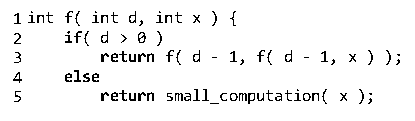
\includegraphics[width=1.0\textwidth]{Code/just_calling_benchmark}
        \caption{The microbenchmark for measuring call frame allocation overhead.}
        \label{fig:micro_calling}
    \end{minipage}\hfill
    \begin{minipage}[t]{0.47\textwidth}
        \centering
        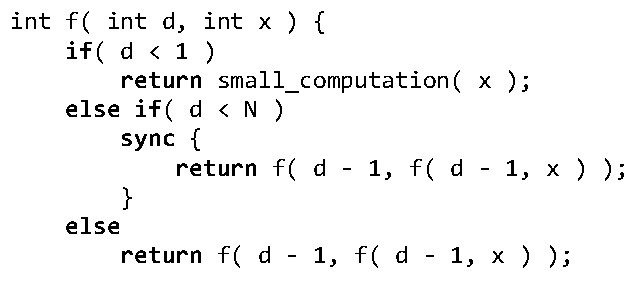
\includegraphics[width=1.0\textwidth]{Code/just_calling_n_benchmark}
        \caption{The call{\slash}return microbenchmark modified to make some calls in sync mode.}
        \label{fig:micro_calling_n}
    \end{minipage}
\end{figure}

(3) Most importantly, all the calls in the first version of this test were performed in interruptible mode.
In sync mode, calls and returns in \charcoal{} are just as efficient as plain C.
In well-tuned \charcoal{} code, most of the short-lived calls should be performed in sync mode.
To simulate this effect, we modified the benchmark to the version in Figure \ref{fig:micro_calling_n}.
The parameter \texttt{N} controls how deep in the call tree the benchmark uses interruptible mode, before switching to sync.


\begin{figure}
    \centering
    \begin{minipage}[t]{0.47\textwidth}
\begin{tabular}{|l|r|r|r|}
  \hline
   & user & sys & wall \\
  \hline
  \hline
  Plain C & 0.77 & 0.00 & 0.77 \\
  \hline
  gcc split stacks\footnotemark{} & 1.00 & 0.15 & 1.15 \\
  \hline
  Go & 2.80 & 0.20 & 3.00 \\
  \hline
  Hot Stacking, \texttt{N} = 4 & 11.00 & 0.01 & 11.00 \\
  \hline
  Hot Stacking, \texttt{N} = 8 & 1.54 & 0.00 & 1.55 \\
  \hline
\end{tabular}

        \caption{Results from the modified call{\slash}return microbenchmark.
      These numbers are in nanoseconds per call{\slash}return.}
        \label{fig:hot_stacking}
    \end{minipage}\hfill
    \begin{minipage}[t]{0.47\textwidth}

\begin{tabular}{|l|r|}
  \hline
  Plain C & 430 \\
  \hline
  \charcoal, \texttt{YIELD\_FREQ = 4} & 1070 \\
  \hline
  \charcoal, \texttt{YIELD\_FREQ = 8} & 519 \\
  \hline
  \charcoal, \texttt{YIELD\_FREQ = 12} & 446 \\
  \hline
\end{tabular}

        \caption{Microseconds per \texttt{strcmp} of two identical strings of 1MB length.}
        \label{fig:strcmp_data}
    \end{minipage}
\end{figure}

\footnotetext{This benchmark does not create stacks deep enough to exceed the default size of a single segment of gcc's split stack.
So we modified the benchmark for the split stack case to make a linear chain of calls instead of a binary tree.}

Figure \ref{fig:hot_stacking} shows that with a modest fraction of the (static) calls performed in sync mode, the calling overhead gets down to less than a factor of 2.
Combined with the observations above about implementation tuning, this overhead would be barely noticeable for most applications.
Also it is worth noting that this is the price to be paid for the extremely low memory overhead of hot stacking.

Hot stacking with \texttt{N} = 8 outperforms Go on this benchmark by a modest margin.
It is interesting that the gap between plain C and Go is as large as it is, given the Go implementation team's famous focus on low-level performance details.

gcc's split stack implementation outperforms hot stacking by a small margin on this benchmark.
However, as noted previously split stacks have bad performance in the pathological case where calls are made at high frequency right at the edge of a segment.

\subsection{Yielding}

In many cases the performance of the yield{\slash}await primitive is unimportant.
Generally hot inner loops should be running in sync mode where yields can be optimized out entirely.
In most non-inner loop code a few extra instructions here or there is barely noticeable.

There are a few cases that do not fit nicely into one of these extremes.
For example, the \texttt{strcmp} function from the C standard library.
\texttt{strcmp} is tricky for a few reasons:
First, the input strings can be arbitrarily long, so never yielding could cause unresponsiveness.
Second, the body of the loop is extremely simple; good implementations are just a few assembly instructions.
This means that yielding every iteration causes significant performance overhead.
Third, the continued execution of the loop depends on the data read in each iteration, so loop tiling{\slash}blocking tricks do not work.
The best-performing implementation we have found so far appears in Figure \ref{fig:strcmp}.


%% \begin{figure}
%%     \centering
%%     \begin{subfigure}[b]{0.3\textwidth}
%%         \hspace{-1.5cm}
%%         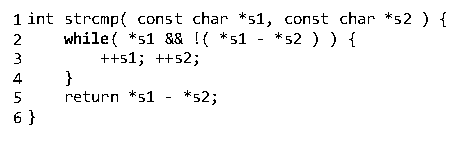
\includegraphics{plain_strcmp}
%%         \caption{}
%%     \end{subfigure}
%%     ~ %add desired spacing between images, e. g. ~, \quad, \qquad, \hfill etc. 
%%       %(or a blank line to force the subfigure onto a new line)
%%     \begin{subfigure}[b]{0.3\textwidth}
%%         \hspace{-1.5cm}
%%         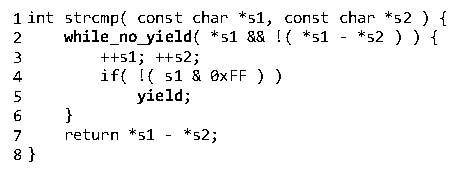
\includegraphics{strcmp_benchmark}
%%         \caption{}
%%     \end{subfigure}
%%     \caption{Two implementations of \texttt{strcmp}.
%%       (a) is a plain C version.
%%       (b) is a \charcoal{} implementation aimed at minimizing yield overhead. }
%%     \label{fig:strcmp}
%% \end{figure}

In the code, \texttt{YIELD\_FREQ} controls how frequently the loop yields.
The effect is that once every $2^{\mathtt{YIELD\_FREQ}}$ iterations there is a yield.
Figure \ref{fig:strcmp_data} shows that yielding is not zero-overhead, but with a little careful tuning the yield overhead can be brought quite low.

When the inputs to \texttt{strcmp} are known to be short, the caller can wrap the call in sync.
The sync version should perform identically to the plain C implementation.

\begin{figure}
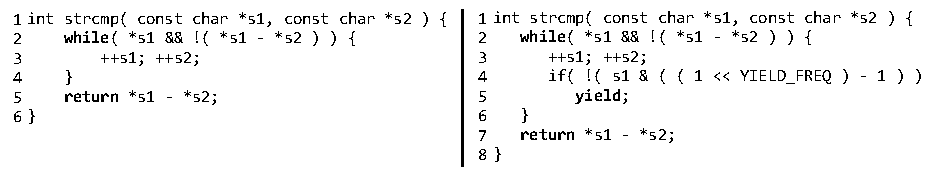
\includegraphics[width=0.99\textwidth]{Code/strcmps}
\caption{Two implementations of \texttt{strcmp}.
  Left is a plain C version.
  Right is a \charcoal{} implementation aimed at minimizing yield overhead.}
\label{fig:strcmp}
\end{figure}

% \subsection{Code Size}

\subsection{Microbenchmark Summary}

Like all well implemented coroutines, the \charcoal{} implementation has extremely low memory and time overhead for basic concurrency primitives.
Hot stacking and frequent yielding are potential performance issues, but our tests indicate that at these overheads can be managed.

Though we do not have experience with writing large programs in \charcoal{} yet, we expect that relatively little code will require the kinds of contortions shown in the \texttt{strcmp} example.
Moreover, almost all such code will be in tight inner loops in library code.
This is exactly where writing somewhat weird code for performance reasons is acceptable.

\section{Summary}

A generation ago there was a debate about whether event loops or threads were better for writing multitasking code.
Multithreading provided a much more natural code style, but was too bug prone, and event loops became the more common framework in many application domains.

In recent years multitasking patterns have become more complex in many application domains, accentuating the pain of event loop code and prompting many languages to adopt coroutines, which can be seen as a compromise between event loops and preemptive mulltithreading.

In this paper we advocate for continuing this trend from coroutines to cooperative multithreading.
We explore, both empitically and analytically, some of the weaknesses of coroutines.
Most importantly, the fact that atomicity versus interuptibility is baked in to routine versus coroutine definitions leads to awkward duplication of library and application code.

Designers of most popular langauges have avoided cooperative multithreading.
We address two of the potential reasons for this: call frame allocation efficiency and the visibility and controlability of atomic versus interruptible calls.
We believe that these improvements make cooperative multithreading an attractive alternative to coroutines.

% \acks

% Acknowledgments, if needed.

% We recommend abbrvnat bibliography style.

% \bibliographystyle{abbrvnat}
\bibliographystyle{abbrv}

% The bibliography should be embedded for final submission.

\bibliography{charcoal.bib}

%% \begin{thebibliography}{../../../../Documents/PapersForReferencing/biy_all_research.bib}
%% \softraggedright

%% \end{thebibliography}

\end{document}
